\begin{name}
	{\tenchude}{\tendethi}{---vvv---}{\thoigian}
\end{name}
\setcounter{ex}{0}\setcounter{bt}{0}
%Câu 1
\begin{ex}
Cho biểu thức $A=\left(\dfrac{1}{3}\right)^{-3} \cdot 27^2$. Khẳng định nào dưới đây đúng?
\choice
{$A=3^9$}
{$A=3^3$}
{$A=3^6$}
{$A={3^{12}}$}
\end{ex}
%Câu 2
\begin{ex}
Khẳng định nào dưới đây đúng?
\choice
{${{2024}^{\tfrac{2}{3}}}=\sqrt{{{2024}^3}}$}
{${{2024}^{\tfrac{2}{3}}}=\sqrt[3]{{{2024}^2}}$}
{${{2024}^{\tfrac{2}{3}}}={{\left({{2024}^3}\right)}^2}$}
{${{2024}^{\tfrac{2}{3}}}={{\left({{2024}^2}\right)}^3}$}
\end{ex}
%Câu 3
\begin{ex}
Kết luận nào đúng về số thực $a$ nếu ${a^{-\dfrac{1}{24}}}>{a^{-\dfrac{1}{15}}}$
\choice
{$a>1$}
{$a<1$}
{$0<a<1$}
{$1<a<2$}
\end{ex}
%Câu 4
\begin{ex}
Cho biểu thức $P=\dfrac{{a^{\sqrt{11}+2}} \cdot {a^{1-\sqrt{11}}}}{{{\left({a^{\sqrt{3}-2}}\right)}^{\sqrt{3}+2}}}$ với $a>0$. Rút gọn biểu thức $P$ được kết quả
\choice
{$P=a^5$}
{$P=a^3$}
{$P=a$}
{$P=a^4$}
\end{ex}
%Câu 5
\begin{ex}
Giá trị của biểu thức $A={{\log _23 \cdot \log _34 \cdot \log _45 \cdot \cdot \cdot \log }_{63}}64$ bằng
\choice
{$6$}
{$7$}
{$8$}
{$10$}
\end{ex}
%Câu 6
\begin{ex}
Xét tất cả các số thực dương $a,b$ thỏa mãn $\log _2a+\log _8b=1$. Mệnh đề nào dưới đây đúng?
\choice
{$ab=2$}
{$a^3b=1$}
{$ab^3=2$}
{$a^3b=8$}
\end{ex}
%Câu 7
\begin{ex}
Với $a$ và $b$ là hai số thực dương tùy ý, $\log \left(ab^2\right)$ bằng
\choice
{$2\log a+\log b$}
{$\log a+2\log b$}
{$2\left(\log a+\log b\right)$}
{$\log a+\dfrac{1}{2}\log b$}
\end{ex}
%Câu 8
\begin{ex}
Với $a$ là số thực dương tùy ý, $\ln (5a)-\ln (3a)$ bằng
\choice
{$\dfrac{\ln (5a)}{\ln (3a)}$}
{$\dfrac{\ln 5}{\ln 3}$}
{$\ln \dfrac{5}{3}$}
{$\ln (2a)$}
\end{ex}
%Câu 9
\begin{ex}
Trong các hàm số sau, hàm số nào đồng biến trên $\mathbb{R}$?
\choice
{$y=\left(\dfrac{2}{e}\right)^x$}
{$y={{\left(\dfrac{\pi }{4}\right)}^x}$}
{$y={{\left(\dfrac{1}{3}\right)}^x}$}
{$y={{\left(\dfrac{\pi }{3}\right)}^x}$}
\end{ex}
%Câu 10
\begin{ex}
\immini{Đồ thị dưới đây là đồ thị của hàm số nào trong 4 đáp án sau:
\choice
{$y=2x^2$}
{$y=3^x$}
{$y=4^x$}
{$y=2^x$}}
{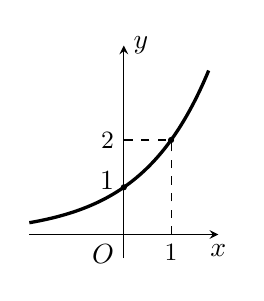
\begin{tikzpicture}[smooth,samples=300,scale=0.6,>=stealth]
			\draw[->] (-2,0)--(2,0) node[below]{$x$};
			\draw[->] (0,-0.5)--(0,4) node[right]{$y$};
			\draw (0,0) node[below left]{$O$};
			\draw[line width=1.2pt,domain=-2:1.8] plot(\x,{2^(\x)});
			\draw[fill=black] (0,1) circle(1.5pt) (1,2) circle(1.5pt);
			\draw[dashed] (1,0)node[below]{\small $1$}--(1,2)--(0,2)node[left]{\small $2$};
			\node[left] at (0,1.15) {$1$};
		\end{tikzpicture}}
\end{ex}
%Câu 11
\begin{ex}
Áp suất không khí $P$(đo bằng $mmHg$) giảm theo độ cao $x$(đo bằng $m$) tại khu vực đỉnh Fansipan của Việt Nam được tính theo công thức: $P=P_0 \cdot {e^{x \cdot i}}$. Trong đó $P_0=760mmHg$ là áp suất ở mực nước biển ứng với $x=0$ và $i$ là hệ số suy giảm áp suất. Biết rằng ở độ cao $1000m$ thì áp suất của không khí là $668mmHg$. Hỏi áp suất của không khí tại đỉnh Fansipan bằng bao nhiêu biết rằng đỉnh Fansipan ở độ cao $3140m$ so với mực nước biển?
\choice
{$502{,}58(mmHg)$}
{$508{,}25(mmHg)$}
{$505{,}28(mmHg)$}
{$500{,}5(mmHg)$}
\end{ex}
%Câu 12
\begin{ex}
Có bao nhiêu số nguyên $x>0$ để hàm số $y=\log_{2023}(2024-x)$ xác định.
\choice
{$2024$}
{$0$}
{Vô số}
{$2023$}
\end{ex}
%Câu 13
\begin{ex}
Cho hàm số $y={{\log }_{2023-2a}}x$ với a là tham số. Có bao nhiêu số tự nhiên a để hàm số đã cho đồng biến trên $\left(0;+\infty\right)$?
\choice
{$1011$}
{$2023$}
{$2022$}
{$0$}
\end{ex}
%Câu 14
\begin{ex}
Để đặc trưng cho độ to nhỏ của âm, người ta đưa ra khái niệm mức cường độ của âm. Một đơn vị thường dùng để đo mức cường độ của âm là đềxinben (viết tắt là $\text{dB}$). Khi đó mức cường độ $L$ của âm được tính theo công thức:$L=10\text{log}\dfrac{I}{I_0}$ trong đó, $I$ là cường độ của âm tại thời điểm đang xét, $I_0$ cường độ âm ở ngưỡng nghe$\left(I_0=10^{-12}\,\text{w}/{{\text{m}}^2}\right)$. Có hai cây đàn ghita giống nhau, cùng hòa tấu một bản nhạc. Biết rằng mỗi chiếc đàn phát ra âm có mức cường độ âm trung bình là $60\text{dB}$. Hỏi mức cường độ âm tổng cộng bằng bao nhiêu?
\choice
{$120\,\text{dB}$}
{$63\,\text{dB}$}
{$60\,\text{dB}$}
{$90\,\text{dB}$}
\end{ex}
%Câu 15
\begin{ex}
Số nghiệm thực của phương trình $3^x{{ \cdot 5}^{x^2}}=1$
\choice
{$0$}
{$1$}
{$2$}
{$3$}
\end{ex}
%Câu 16
\begin{ex}
Số nghiệm thực của phương trình ${{\left(\sqrt{5}-2\right)}^{\tfrac{2x}{x-1}}}={{\left(\sqrt{5}+2\right)}^x}$ là
\choice
{$0$}
{$1$}
{$2$}
{$3$}
\end{ex}
%Câu 17
\begin{ex}
Thông tin về tình hình dân số, lao động việc làm quý $IV$ và năm $2023$ của Tổng cục Thống kê (Bộ Kế hoạch và Đầu tư) cho biết, dân số trung bình của Việt Nam năm $2023$ đạt $100{,}3$ triệu người với tỉ lệ tăng trưởng dân số $r=0{,}8\%$ một năm. Giả sử nếu tỉ lệ tăng trưởng không thay đổi trong các năm tiếp theo, đến năm bao nhiêu thì dân số Việt Nam sẽ tăng gấp đôi?
\choice
{$2100$}
{$2110$}
{$2120$}
{$2120$}
\end{ex}
%Câu 18
\begin{ex}
Tổng các nghiệm thực của phương trình ${{\log }_{\sqrt{3}}}(x-2)+{{\log _3(x-4)}^2}=0$ là $S=a+b\sqrt{2}$ (với $a,b$ là các số nguyên). Giá trị của biểu thức $S=a+b$ bằng
\choice
{$1$}
{$4$}
{$6$}
{$7$}
\end{ex}
%Câu 19
\begin{ex}
Tích tất cả các nghiệm thực của phương trình $\dfrac{1}{2}\log \left(x^2-4x-1\right)=\log 2x-\log x$ bằng
\choice
{$-5$}
{$3$}
{$5$}
{$1$}
\end{ex}
%Câu 20
\begin{ex}
Tập nghiệm của bất phương trình ${{2 \cdot 3}^{x+1}}\le {2^{2x+3}}$ là
\choice
{$S=\left(-\infty ;-1\right]$}
{$S=\left[-1;+\infty\right)$}
{$S=\left(-\infty ;1\right]$}
{$S=\left[1;+\infty\right)$}
\end{ex}
%Câu 21
\begin{ex}
Giải bất phương trình ${\left(\dfrac{1}{2024}\right)}^{-2023x+1}>2024^{2022}$ ta được tập nghiệm là
\choice
{$S=\left(-\infty ;1\right)$}
{$S=\left(-\infty ;-1\right)$}
{$S=\left(1;+\infty\right)$}
{$S=\left(-1;+\infty\right)$}
\end{ex}
%Câu 22
\begin{ex}
Tập nghiệm $S$ của bất phương trình ${{\ln }^2}x-2023\ln x-2024\ge 0$ là
\choice
{$S=\left(0;\dfrac{1}{e}\right]\cup \left[{e^{2024}};+\infty\right)$}
{$\left[{e^{2024}};+\infty\right)$}
{$\left[{e^{2024}};+\infty\right)$}
{$S=\left(-\infty ;\dfrac{1}{e}\right]\cup \left[{e^{2024}};+\infty\right)$}
\end{ex}
%Câu 23
\begin{ex}
Cho bất phương trình $e^x-2024 \cdot e^x+2023\le 0$. Số giá trị nguyên của $x$ thỏa mãn bất phương trình đã cho là:
\choice
{$5$}
{$6$}
{$7$}
{$8$}
\end{ex}
%Câu 24
\begin{ex}
Một người gửi 100 triệu đồng vào ngân hàng với lãi suất $6\%/$ năm. Biết rằng nếu không rút tiền khỏi ngân hàng thì cứ sau mỗi năm, số tiền lãi sẽ được nhập vào vốn ban đầu để tính lãi cho năm tiếp theo. Hỏi sau ít nhất bao nhiêu năm người đó nhận được số tiền nhiều hơn 200 triệu đồng bao gồm cả gốc và lãi? Giả sử trong suốt thời gian gửi lãi suất không đổi và người đó không rút tiền ra.
\choice
{$11$ năm}
{$12$ năm}
{$13$ năm}
{$10$ năm}
\end{ex}
%Câu 25
\begin{ex}
Huyện A có $300$ nghìn người. Với mức tăng dân số bình quân $1{,}2\%$/năm thì sau $n$ năm dân số sẽ vượt lên $330$ nghìn người. Hỏi $n$ nhỏ nhất bằng bao nhiêu?
\choice
{8 năm}
{9 năm}
{7 năm}
{10 năm}
\end{ex}
%Câu 26
\begin{ex}
Trong vật lí, sự phân rã của các chất phóng xạ được biểu diễn bởi công thức: $m(t)={{m_0\left(\dfrac{1}{2}\right)}^{\tfrac{t}{T}}}$, trong đó $m_0$ là khối lượng ban đầu của chất phóng xạ (tại thời điểm t = 0); T là chu kì bán rã (tức là khoảng thời gian để một nửa khối lượng chất phóng xạ bị biến thành chất khác). Chu kì bán rã của Cabon $^{14}C$ là khoảng 5730 năm. Người ta tìm được trong một mẫu đồ cổ một lượng Cabon và xác định được nó đã mất khoảng 25\% lượng Cabon ban đầu của nó. Hỏi mẫu đồ cổ đó có tuổi gần nhất với số năm nào?
\choice
{2400 năm}
{2300 năm}
{2387 năm}
{2378 năm}
\end{ex}
%Câu 27
\begin{ex}
Một nghiên cứu cho thấy một nhóm học sinh được cho xem cùng một danh sách các loài động vật và được kiểm tra lại xem họ nhớ bao nhiêu \% mỗi tháng. Sau t tháng, khả năng nhớ trung bình của nhóm học sinh được cho bởi công thức $M(t)=75-20\ln (t+1),t\ge 0$ (đơn vị \%). Hỏi sau ít nhất bao nhiêu tháng thì nhóm học sinh nhớ được danh sách đó dưới 10\%?
\choice
{25 tháng}
{23 tháng}
{24 tháng}
{22 tháng}
\end{ex}
%Câu 28
\begin{ex}
Cho hình lập phương $ABCD \cdot A'B'C'D'$. Góc giữa hai đường thẳng $BA'$ và $C'D'$ bằng: 
\choice
{$45^\circ $}
{$60^\circ $}
{$30^\circ $}
{$90^\circ $}
\end{ex}
%Câu 29
\begin{ex}
Cho hình chóp $S \cdot ABCD$ có $SB=SC=SD=BC=CD=DB$. Gọi $I$ là trung điểm của $SD$. Khi đó cosin của góc giữa hai đường thẳng $SB$ và $CI$ bằng?
\choice
{$cos(SB$, $CI)=\dfrac{1}{2}$}
{$cos(SB$, $CI)=\dfrac{\sqrt{3}}{2}$}
{$cos(SB$, $CI)=\dfrac{\sqrt{3}}{4}$}
{$cos(SB$, $CI)=\dfrac{\sqrt{3}}{6}$}
\end{ex}
%Câu 30
\begin{ex}
Cho hình hộp $ABCD \cdot A'B'C'D'$. Giả sử tam giác $AB'C$ và $A'DC'$ đều có 3 góc nhọn. Góc giữa hai đường thẳng $AC$ và $A'D$ bằng góc nào sau đây?
\choice
{$\widehat{AB'C}$}
{$\widehat{BDB'}$}
{$\widehat{BB'D}$}
{$\widehat{DA'C'}$}
\end{ex}
%Câu 31
\begin{ex}
Cho hình chóp $S \cdot ABCD$ có đáy $ABCD$ là hình thoi tâm $O$, $SA\,\bot (ABCD)$. Trong các khẳng định sau, khẳng định nào sai?
\choice
{$SA\bot BD$}
{$SC\bot BD$}
{$SO\bot BD$}
{$AD\bot SC$}
\end{ex}
%Câu 32
\begin{ex}
Ở các thành phố lớn để giảm tình trạng tắc nghẽn giao thông và nhằm đảm bảo an toàn thì ở các ngã tư người ta thường xây dựng các cầu vượt dành cho người đi bộ. Hỏi những phương tiện tham gia giao thông phải có chiều cao như thế nào để di chuyển an toàn bên dưới cầu vượt. Biết rằng đường dẫn lên cầu dài 15 mét và hợp với đường một góc 300?
\choice
{Bằng $5$ mét}
{Nhỏ hơn$7{,}5$ mét}
{Bằng $7{,}5$ mét}
{Nhỏ hơn $5$ mét}
\end{ex}
%Câu 33
\begin{ex}
Cho hình chóp tứ giác đều $S.ABCD$ tâm $O$ có cạnh đáy bằng $2a$ và $SO=a$. Tính góc nhị diện $\left[S, CD, O\right]$.
\choice
{$90^\circ $}
{$45^\circ $}
{$30^\circ$}
{$60^\circ $}
\end{ex}
%Câu 34
\begin{ex}
Cho hình chóp $S \cdot ABC$ có đáy là tam giác vuông cân tại $C$, $BC=a$, $SA$ vuông góc với mặt phẳng đáy và $SA=a$. Khoảng cách từ $A$ đến mặt phẳng $(SBC)$ bằng
\choice
{$\sqrt{2}a$}
{$\dfrac{\sqrt{2}a}{2}$}
{$\dfrac{a}{2}$}
{$\dfrac{\sqrt{3}a}{2}$}
\end{ex}
%Câu 35
\begin{ex}
Cho hình chóp $S \cdot ABCD$ có đáy là hình chữ nhật $AB=a$, $BC=2a$, cạnh bên $SA$ vuông góc với đáy. Khoảng cách giữa hai đường thẳng $SA$ và $CD$ bằng
\choice
{$a\sqrt{6}$}
{$a\sqrt{5}$}
{$a$}
{$2a$}
\end{ex}
%Câu 36
\begin{ex}
Giải phương trình $\log \left(x^2+3\right)=\log (3x+1)$
\end{ex}
%Câu 37
\begin{ex}
Cho $a,b$ là các số thực dương khác $1$ và thỏa mãn: $\ln a+\ln (8b)=2\ln (a+2b)$.
Rút gọn biểu thức $P={{\log _b2a+\log }_{\tfrac{a}{2}}}2b-\dfrac{1}{\log _8b}$
\end{ex}
%Câu 38
\begin{ex}
Cho hình chóp $S \cdot ABCD$ có đáy $ABCD$ là hình vuông cạnh $a$, $SA=a$ và $SA$ vuông góc với mặt đáy. Gọi $M$ là trung điểm của $SD$.\\ 
a) Chứng minh rằng $BD\bot (SAC)$.\\
b) Tính khoảng cách giữa hai đường thẳng $SB$ và $CM$\\
\end{ex}
%Câu 40
\begin{ex}
Giải phương trình $\log _2\left(x-\sqrt{x^2-1}\right) \cdot \log _3\left(x+\sqrt{x^2-1}\right)=\log _6\left| x-\sqrt{x^2-1} \right|$
\end{ex}
